\section*{Two key aspects of file system (data structures \& access methods)}
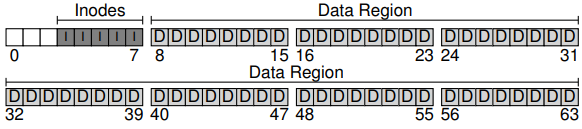
\includegraphics[width=\linewidth]{imgs/fs_simple_blocks1}
\begin{itemize}
\item divide disk into \textbf{blocks}: each of size 4KB, addressed from 0 to $N-1$
\item assume $N=64$ and low-level R/W ops on blocks already implemented
\item \textbf{data region}: region of disk used for user data; assume $N_{\text{data}} = 56$
\item assume $N_{\text{inode}}=5$ and $S_{\text{inode}}=256$B $\to$ 4KB block holds 16 inodes and fs contains 80 in total (max \# of files can be stored in this fs)
\item fs should have
  \begin{enumerate*}[label={\alph*.},font={\color{red!50!black}\bfseries}]
  \item data bloks (D)
  \item inodes (I)
  \item \mb{allocation structures}: bitmap(d,i) for D,I $\to$  free: 0; in-use: 1 (a bit overkill in this case)
\end{enumerate*}
\item \textbf{S}uperblock contains info:
  \begin{enumerate*}[label={\alph*.},font={\color{red!50!black}\bfseries}]
  \item $N_{\text{inodes}}=80; N_{\text{data}} = 56$
  \item inode table begins at block3
  \item magic number (enum) of fs type (vsfs)
  \item other info
\end{enumerate*}
\end{itemize}
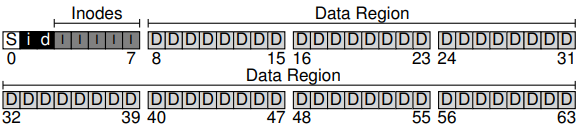
\includegraphics[width=\linewidth]{imgs/fs_simple_blocks2}
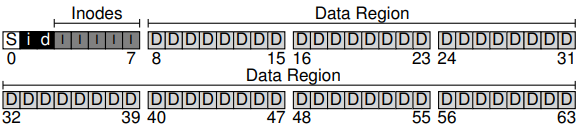
\includegraphics[width=\linewidth]{imgs/fs_simple_blocks2}
\begin{itemize}
\item each inode implicitly pointed to by i-number (low-level name of a file)
\item inode table starts at 12KB and $S_{\text{indtb}} = 20$KB (5 4KB blocks)
\item disks are \emph{not} byte addressable but sector (e.g. 512B) addressable
\begin{lstlisting}[language=c,framextopmargin=-2pt,framexbottommargin=-2pt]
blk = (inumber * sizeof(inode_t)) / blockSize;
sector = ((blk * blockSize) + inodeStartAddr) / sectorSize;
\end{lstlisting}
\item metadata inside each inode:
  \begin{enumerate*}[label={\alph*.},font={\color{red!50!black}\bfseries}]
  \item type (\texttt{-,d,l})
  \item size (\# of blks allocated)
  \item protection info (ownership, access)
  \item time info, etc
\end{enumerate*}
\item each \mo{inode} can contain $\geq 1$ \mb{direct pointers} (disk addresses); each pointer refers to one disk block that belongs to the file
\item drawback: cannot support very large file $\because S \leq S_{\text{blk}} \times$ \texttt{num\_direct\_ptr}
\end{itemize}
\section*{Multi-level Index to support bigger files}
\begin{itemize}
\item \mb{indirect pointer} points to indirect blk containing more ptrs: each points to usr data: an inode with fixed \# of direct ptrs + 1 indirect ptr
\item If a file grows large enough, an indirect blk allocated (from data region) and the inode’s slot for an indirect pointer is set to point to it
\item assume 4KB block and 4B disk addr $\to N_{\text{ptr/blk}} = \frac{4KB}{4B} = 1024$
\item a file can grow to be $(12 + 1024) \cdot 4K = 4144KB$
\item \mb{double indirect pointer} refers to a block that contains pointers
to indirect blocks, each of which contain pointers to data blocks $\to$ files can grow to $(12 + 1024 + 1024^{2}) \times 4KB \approx 4GB$
\item \mb{triple indirect pointer} points to a blk that contains double indirect ptrs
\end{itemize}
\begin{minipage}{.5\linewidth}
  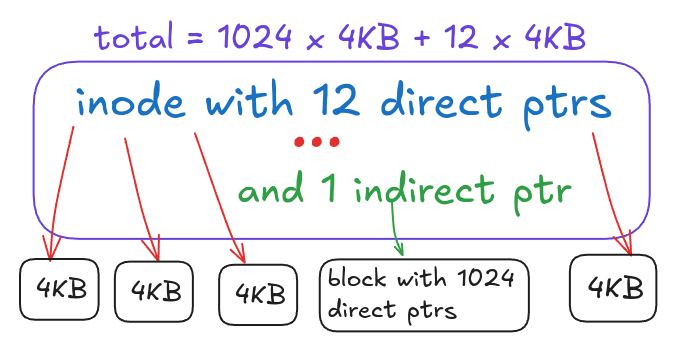
\includegraphics[width=\linewidth]{imgs/fs_indirect_ptr1}
\end{minipage}
\begin{minipage}{.5\linewidth}
  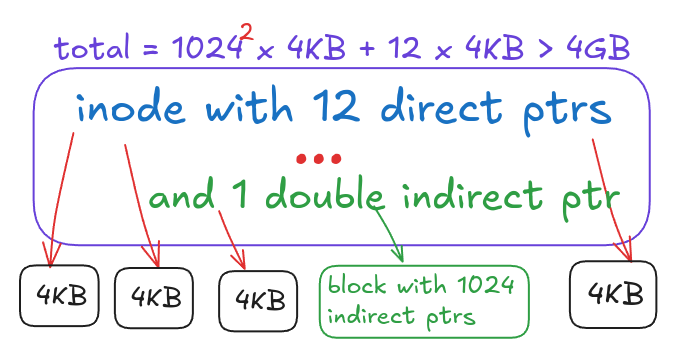
\includegraphics[width=\linewidth]{imgs/fs_indirect_ptr2}
\end{minipage}
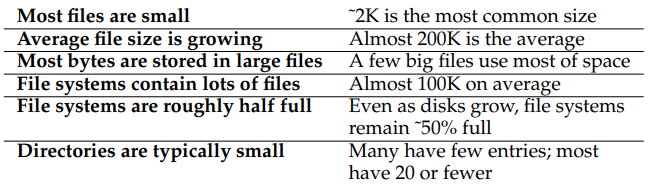
\includegraphics[width=\linewidth]{imgs/fs_measure_sum}
\begin{itemize}
\item most files are small $\to$ can optimize the imbalanced tree (left)
\item typical inode has 12 dirct ptrs + $\geq 1$ indirect blocks for larger files
\end{itemize}
\section*{Directory Organization}
\begin{itemize}
\item filsys treats dirs as special type of file (\texttt{d}): represented in same way as files, with data blks pointed to by inode and perhaps indirect blks
\item XFS uses B-tree, faster than lists, file/dir name must be unique
\item simple org: a dir contains a list of (entry name, inode number) pairs
\item dir has a str + a number in data blks: each str may have variable len
\item
\end{itemize}
\begin{tabular}{l|l|l|l|l}
  inum & reclen & strlen  & name        & note \\
  5    & 12     &  2      & \texttt{.}  & (current dir)\\
  2    & 12     &  3      & \texttt{..} & (parent dir)\\
  12    & 12     &  4      & \texttt{foo}&\\
  13    & 12     &  4      & \texttt{bar}&\\
  24    & 36     & 28      & \texttt{foobar\_is\_a\_pretty\_longname}&\\
  \multicolumn{5}{l}{record len: total bytes for the name + any leftover space (`$\backslash$0' included)}\\
  \hline
  \multicolumn{5}{l}{deleting a file $\to$ empty space in middle of dir and should be marked}\\
  \multicolumn{5}{l}{new entry reuses old, bigger entry $\therefore$ extra space within and reclen is used}\\
\end{tabular}
\section*{Access Paths: Reading and Writing (assume filesize 12KB, blksize 4KB)}
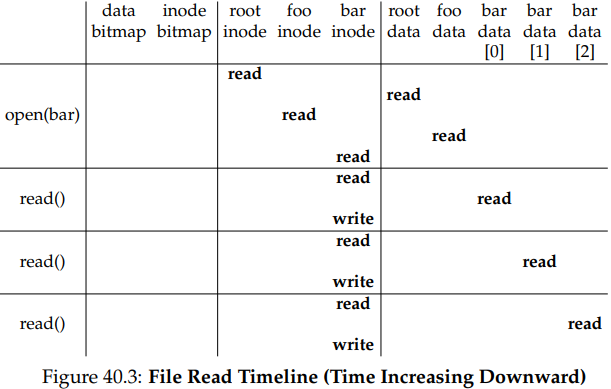
\includegraphics[width=\linewidth, height=5.5cm]{imgs/fs_read_timeline}
\begin{itemize}
\item issue \texttt{open("/foo/bar",O\_RDONLY)} $\to$ filesys needs to find inode for \texttt{bar}
\item filesys only knows \mo{root} inumber: 2 by default; must \mo{traverse} pathname
\item read into root, find ptrs to data blocks, look for \texttt{foo} entry inumber
\item recursively traverse until desired inode found $\to$ \texttt{bar} inode into RAM
\item Once open, \texttt{read()} starts at offset 0 unless \texttt{lseek()} already called
\item read 1st block \& update
  \begin{enumerate*}[label={\arabic*.},font={\color{red!50!black}\bfseries}]
  \item $T_{\text{last-accessed}}$
  \item RAM OFT for this fd
  \item file offset $\to$ next read will read the second file block
  \end{enumerate*}
\item \texttt{close()}, deallocated fd, no disk I/O for closing file in this case
\item amount of I/O by open is \mr{proportional} to the length of the pathname
\item must read inode and data for each additional directory in the path
\item large dirs: read many data blks to find target entry $\to$ perfermance $\downarrow$
\item \texttt{open()} and \texttt{write()} $\to$ may allocate new block (unless overwriting)
\item each write
  \begin{enumerate*}[label={\arabic*.},font={\color{red!50!black}\bfseries}]
  \item decide which blk to alloc to the file, update other disk struct (bitmap, inode, etc)
  \item write data to disk
  \end{enumerate*}
\item 1 write $\to$ 5 I/Os:
  \begin{enumerate*}[label={\arabic*.},font={\color{red!50!black}\bfseries}]
  \item read bitmap; mark new alloc
  \item write new bitmap back to disk
  \item 2 more: read and write the inode
  \item write actual block
  \end{enumerate*}
\item create file: \textbf{10} I/Os and each alloc causes \textbf{5} I/Os:
  \begin{enumerate*}[label={\arabic*.},font={\color{red!50!black}\bfseries}]
  \item a pair to read/update the inode
  \item a pair to read/update the bitmap
  \item write data
  \end{enumerate*}
\end{itemize}
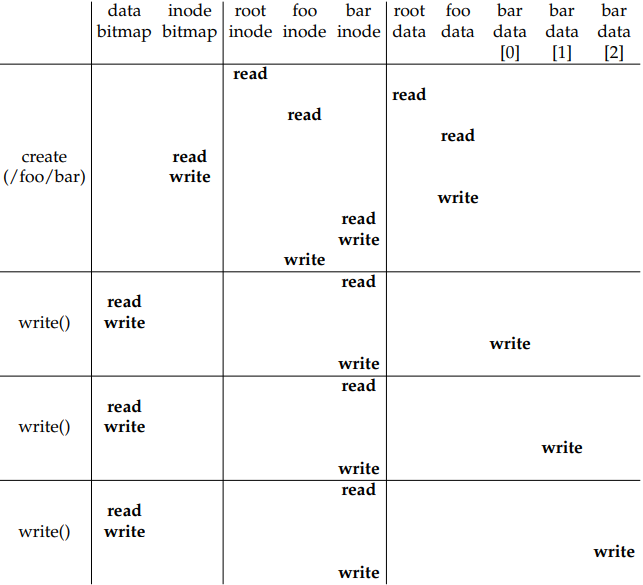
\includegraphics[width=\linewidth, height=7.5cm]{imgs/fs_write_timeline}
\section*{Caching and Buffering (modern filesys buffer Ws in RAM for 5-30s)}
\begin{itemize}
\item fixed-size cache to hold popular blocks and LRU to decide to keep which
\item fixed-size cache usually allocated at boot time; $\approx 10\%$ of total RAM
\item \mb{static partitioning}: wasteful, unable to re-purpose unused space; ensures each user receives some share of resource, usually delivers more predictable performance, often easier to implement
\item modern OS: \mb{dynamic partitioning} + virtual RAM: unified page cache; better utilization (by letting resrc-hungry users consume otherwise idle resrc); more complex to implement; can lead to worse perf. if one's idle resrc get consumed by others and need to take long time to reclaim
\item 1st open causes many I/Os; subsequent same file/dir opens hit cache
\item write has to put data to disk (persistent) so cache no longer serves
\item buffering write has benefits:
  \begin{enumerate*}[label={\arabic*.},font={\color{red!50!black}\bfseries}]
  \item filesys can batch updates into smaller set of I/Os: create file1 and later create file2 $\to$ update inode bitmap only once
  \item buffering writes in RAM $\to$ sys can schedule subsequent I/Os $\to$ perfermance $\uparrow$
  \item avoid some unnecessary writes: create a file and then delete it $\to$  avoid them entirely and lazy is good
  \end{enumerate*}
\item if sys crashes before actual writing data to disk, updates lost
\item DBMS usually forces writes to disk (\texttt{fsync()}, direct I/O interface)
\end{itemize}
\begin{tcolorbox}[left=0mm, top=1mm, right=0mm, rightlower=0mm, bottom=1mm,
  title= Reads DON’T access allocation structures,
  halign title=center]
  Allocation structures, such as bitmaps, are only accessed when allocation is needed. The inodes, directories, and indirect blocks have \emph{all} the information they need to complete a read request; there is no need to make sure a block is allocated when the inode already points to it.
\end{tcolorbox}
There needs to be some info about each file (metadata), usually
stored in a struct called an inode. Directories are just a specific type
of file that store name$\to$inode-number mappings. Filesys often use a bitmap to track which inodes/data blks are free/allocated.
